\newtheorem{theorem}{Theorem}[section]
\newtheorem{corollary}{Corollary}
\chapter{Platooning}
The first idea of platooning was published in \cite{shladover1979} with the definition:

\textit{
\newline
Platoon is a collection of vehicles that travel close together, actively coordinated in formation.}
\newline

But this formulation is not as specific as it would be for our situation, so we prefer the definition which is mentioned in SARTRE platooning concept \cite{bergenhem2010challenges}:

\textit{
\newline
A platoon is a number of vehicles that are travelling together and electronically connected. There is one lead vehicle and one or more following vehicles. The following vehicles of a platoon are controlled autonomously while the lead vehicle is controlled manually}
\newline

As it is mentioned in the previous definition, the biggest interest in platooning appeared with the development of electronic communication channels - Vehicle to Vehicle (V2V) and Vehicle to Infrastructure (V2I) based on wireless connection.

This idea enchanted a lot of people all over the world and now there are several projects which are working on this topic. The most known are SARTRE\footnote{\url{http://www.sartre-project.eu/en/Sidor/default.aspx}}  (Europe), PATH\footnote{\url{http://www.path.berkeley.edu/research/automated-and-connected-vehicles/truck-platooning}}  (USA), GCDC\footnote{\url{https://gcdc.net}}  (Germany), SCANIA\footnote{\url{http://www.scania.com}}  (Europa - Japan), Energy ITS\footnote{\url{http://orfe.princeton.edu/~alaink/SmartDrivingCars/ITFVHA13/ITFVHA13_JP_Energy_ITS_Tsugawa.pdf}}  (Japan), AUTO21\footnote{\url{https://www.auto21.ca/en/}}  (Canada) and many others. These projects cannot be described together because they differ in specific parts, but all of them are proving positive effects of platooning concept on highway traffic.

\newpage
\section{Recent research projects overview}

International Europe project SARTRE - Safe Road Trains for the Environment is funded by the European Commission and includes many European science and university institutes and it also cooperates with Volvo research centres. It is a complex solution which includes longitudinal and lateral control of platoons of both types of vehicles (heavy vehicles trucks and passenger vehicles - cars). Vehicles communicate with each other only via V2V communication channel based on ITS-G5 and it means, no changes in highway infrastructure are necessary. Another project which is suitable for mixture of passenger vehicles and trucks is project GCDC, Grand Cooperative Driving Challenge in Germany, which is implementable in urban environment too.

Another group of projects is focused only on trucks. One of such projects is SCANIA in which they are working on safety longitudinal control (lateral movement is manual) without any change on routes. Project Energy ITS is one of the most recent projects which started in 2008. To compare it with the previous one, trucks have automatically a lateral control too, but it assumes lane markings in highway. Very similar to those projects is German KONVOI\footnote{\url{https://www.ika.rwth-aachen.de/pdf_eb/gb6-24e_konvoi.pdf}}  too.

The California (Berkeley) project PATH - Partners for Advanced Transportation Technology belongs into the special category. Its idea allows platooning of passenger vehicles or trucks, these two types of vehicles cannot be mixed. It assumes dedicated lanes with embedded reference markers in the road surface and with this condition the vehicles are able to do longitudinal and lateral control. The most interesting thing and what is totally different from other projects is that even the leading car is fully autonomously controlled.

\section{Lifecycle of platoon}

The concept of platooning has three main lifecycle sections of a platoon. The first section is how the platoon should be created and how to sort vehicles in a platoon, in a convoy. The second section is a task about acting and behaviour on highway and the last section is about leaving the platoon. This thesis is focused on the second one (behaviour) and simulates and analyses the vehicle and platoon behaviour in highway traffic. Below there is a description of all parts of the platoon lifecycle for better understanding of these topics.

\subsection{Formation of platoon}

Every highway entrance ramp or highway entrance ramp lane is a point of decision, which platoon the vehicle will be assigned to, or whether the vehicle will create its own platoon of which it will be the lead vehicle. This decision is based on thresholds how much the vehicle would have to change its speed and what distance is to some already existent platoons driving on highway. 

This part is also important for sorting of vehicles, because only here we can actively manage the order of vehicles in platoons. According to most recent projects – see in references, every vehicle in platoon should be in the order in which they leave the highway and the platoon. It means the last vehicle in the platoon will leave the platoon and the highway as the first  vehicle.

If a vehicle wants to join an existent platoon, other vehicles should create space behind the platoon or the platoon vehicles should create space inside the platoon to provide right position order inside the platoon for the new vehicle.

\subsection{Platoon behaviour on highway}

This part of the platoon lifecycle describes the period between establishing and decomposition of platoon, the period between entering and leaving of the vehicle into or from the platoon; it means that the platoon is moving without changing the numbers of vehicles in the platoon. Changes of platoon content or order are considered as decomposition and establishing of platoon. During this lifecycle period the platoon solves several partial problems, for example how to behave during overtaking, changing of lane, changing of platoon speed and distances between platoon vehicles, etc. or what to do with “problematic” drivers who try to destroy the cooperation of the vehicles that are included in the existent platoon. This second mentioned problem can be solved by changing the distances between the vehicles in the platoon, i.e. reducing the distances so that not “to allow” the other vehicles to get into the platoon and “to destroy” it.

This state, going/being in platoon, is the biggest part of driving on the highway. In this state the vehicles of the platoon stay for most of their time on the highway. So it is not a surprise that most of the optimization must be done there. The distance between the vehicles in the platoon and also the maximum number of vehicles which can be in one platoon have the main influence and are very important for the increase of traffic capacity.

\subsection{Decomposition of platoon}

Leaving the platoon should be the easiest part of platoon lifecycles because at this time the leaving vehicle should be on the last position in the platoon order. So the vehicle only slows down and leaves the platoon and later also the highway or goes into another platoon.

\section{Advantages of platoonig concept}

The main reason of platoon research on highway is to increase lane traffic capacity. It means that more vehicles can pass through a part of highway per a time period, the most common indicator “capacity of lane” is the number of vehicles per hour. So the equation for maximum safety capacity is: 

\begin{equation}\protect\label{eq:max_cap_single}
c_{max}=\frac{3600}{s+t_{s}\cdot v}\cdot v
\end{equation}

where  $c_{max}$  is the maximum capacity of vehicles per lane and per hour to steady state speed $v$ in meters per second, $s$ is the average length of a vehicle in meters and  $t_{s}$ is the time between two vehicles (safety time) in seconds.

For the calculation of maximum capacity of lane with platoons, we have to change the equation into the form which includes more parameters, but it is only a generalization of the Equation \ref{eq:max_cap_single}:

\begin{equation}\label{eq:max_cap_platooning}
c_{max}=\frac{3600\cdot X}{(X-1)\cdot(d+s)+s+t_{s}\cdot v}\cdot v
\end{equation}

where $X$ is the maximum number of vehicles which can be in one platoon and $d$ is the distance between two vehicles of the platoon in meters, distance between vehicles in platoon is constant. It assumes that distance $d$ is a constant for all speed of platoon so there is a space for more optimization but for this thesis this Equation \ref{eq:max_cap_platooning} is sufficient. We can also see that Equation \ref{eq:max_cap_platooning} is the same as Equation \ref{eq:max_cap_single} for  $X=$ 1  which means, platoons consist of one vehicle. Similar equation was published in \cite{dao2013strategy}, but we had to adapt it for our purposes. 

There is a "rule" for safety driving on highways in the Czech Republic which says that there should be a safe distance between two vehicles of the same speed which corresponds to the distance travelled by car for a period of 2 seconds. This is not an official rule, but it is a recommendation given in every driving school.

Let us assume an example with one highway lane in which there is an average speed \mbox{$v$ = 108 km/h} which equals to 30 m/s. Let us set other parameters: \mbox{$t_{s}$  = 2 s} (which corresponds to the recommended safety time in the Czech Republic), \mbox{$s$ = 4 m}, \mbox{$X$ = 5} and \mbox{$d$ = 6 m}. With these conditions the maximum capacity  $c_{max}$   of the highway without platooning concept \mbox{($X$ = 1)} will be 1 687 vehicles per hour and on the other hand the vehicles capable of platooning increase the maximum capacity $c_{max}$ to 5 400 vehicles per hour. This example proves a positive impact of platooning on maximum highway capacity because in optimal conditions platoons of 5 vehicles increase the capacity more than 3 times.

In the following Figure \ref{fig:3_3-1} you can see dependency of average speed in a lane and maximum capacity in the lane for cooperative and non-cooperative vehicles. The rest of variables are the same as in the previous example.

\begin{figure}[!htbp]
\centering
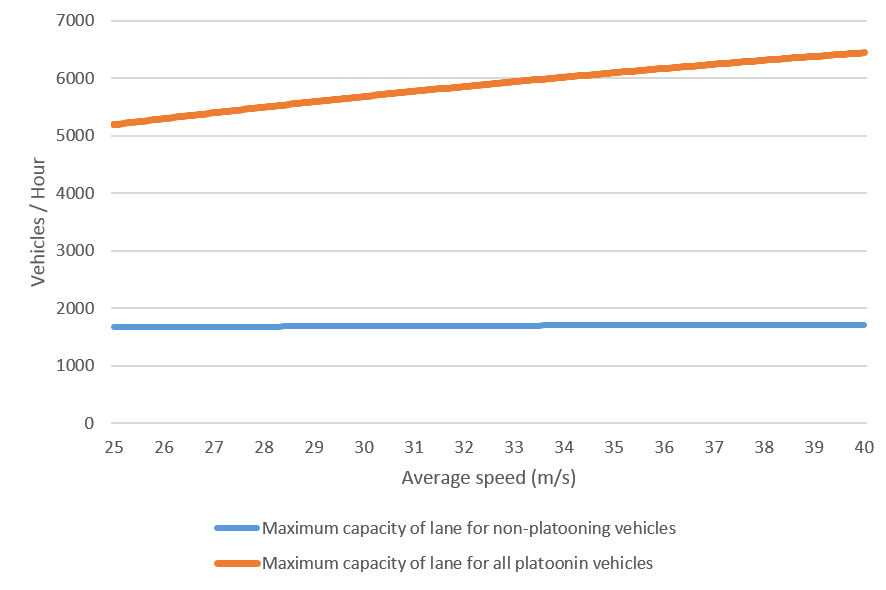
\includegraphics[width=0.90\textwidth,height=0.90\textheight,keepaspectratio]{figures/Chapter_3/3_curve_nonXplatooning_vehicles.png}
\centering
\protect\caption{\label{fig:3_3-1}Maximum capacity of lane for different average speeds}
\end{figure}

The increased capacity of highway is not the only positive effect of this concept. Autonomously controlled vehicles can also help with traffic safety, because of V2V communication, the vehicles can have on-line information about problematic situations and risks, they can react faster and therefore they have a longer time to solve the situation. In case that all vehicles can cooperate together, they can share information  e.g.. about braking and a vehicle can slow down faster than its driver can notice the action.

Another positive result of platooning and its close formation is the possibility to save fuel. Browand and Michaclian\cite{zabat1995estimates}\cite{browand2000platoon} proved that in the platoon of speed 96km/h with distance between vehicles 3 m, every vehicle (except for the leading one) can save from 5\% to 12\% of fuel depending on the type of vehicles. As an additional austerity result of this approach, it also decreases the amount of emission of $CO_{2}$ up to 2\%

\section{Disadvantages of platooning concept}

Concept of platooning is based on autonomous controlled vehicles, so there is a problem of responsibility for accidents which are caused by not human control. But this issue is not a matter of this thesis. Another problem is different level of driver’s knowledge and experiences. The first driver has to do the hardest work, because he has to lead the platoon  although he has no benefit of fuel savings. In agents technologies, this problem is called unfairness.

\section{Platoon rules}

In this part we describe the platooning concept which will be used in this thesis. The platoon consists of vehicles (up to maximum number) and “only” the first one is controlled by human driver, let us call the vehicle as Lead vehicle (LV). LV is equipped with some kind of driving assistant which helps to the driver and with an emergency assistant which can take control during emergency situations. So such a vehicle driver should have better driving skills. The rest of the vehicles are called Following Vehicles (FV) and they could be controlled automatically. Example of platoon you can see in next Figure \ref{fig:3_5-1}.

\begin{figure}[!htpb]
\centering
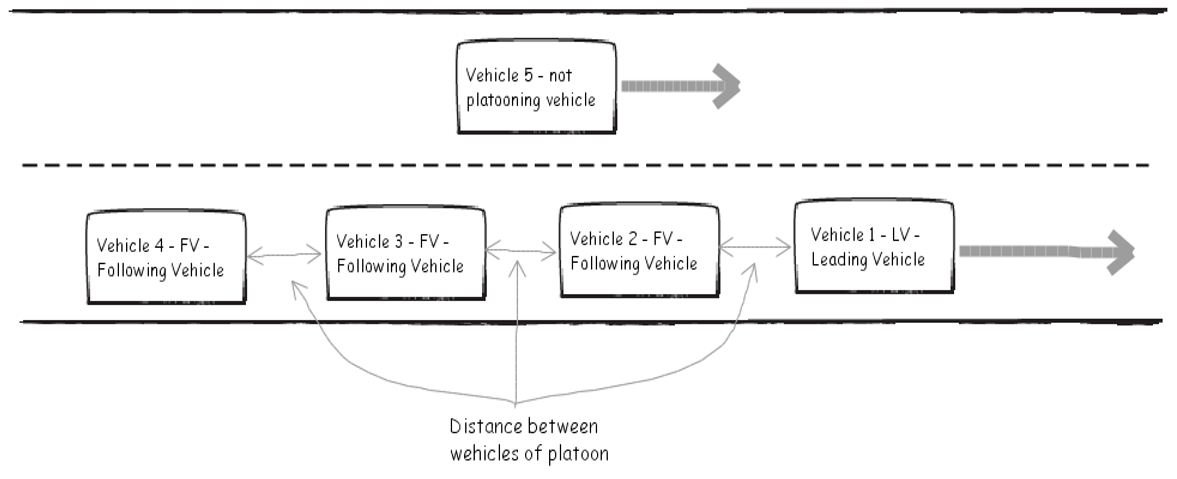
\includegraphics[width=0.90\textwidth,height=0.90\textheight,keepaspectratio]{figures/Chapter_3/3_platoonin_example.png}
\centering
\protect\caption{\label{fig:3_5-1}Example of structure of platoon of 4 vehicles}
\end{figure}

Each vehicle that is able to cooperate is equipped with V2V communication equipment and radar which provides information about all vehicles in reasonable range. So every platoon vehicle can check whether the neighbour lane is free to move there or whether the LV is in safe distance to the vehicle which is in front of it.

Every platoon has its constant preferred speed which can be increased only in case of overtaking a vehicle the speed of which is very similar to the speed of the platoon. This can be done so as not to block the faster lane for a long time. The platoon also changes its speed in problem situations such as traffic jam or traffic accident.

Every auto-controlled FV keeps distance at least 5 m to the front vehicle, but the distance can be changed for some operation of the platoon. For more safety the safe distance time of LV could be increased from 2s to 3s because in case of a collision of LV, every FV will have the collision too (it is not implemented in our simulator).